\documentclass[assign]{article}

\usepackage{graphicx}
\usepackage{amsmath,amssymb,amsthm} % define this before the line numbering.
\usepackage{color}
\usepackage{eso-pic}
\usepackage{bm}
\usepackage{caption}
\usepackage{picins}   
\usepackage{microtype}
\usepackage[mediumspace,mediumqspace,Grey,squaren]{SIunits}
\usepackage{multirow}
\usepackage{epstopdf}
\usepackage[boxed,lined,algonl]{algorithm2e}
\usepackage{url}
\usepackage{enumerate}

% Declaring commonly used math operators
\DeclareMathOperator{\ddiag}{Diag}
\DeclareMathOperator{\rrank}{rank}
\DeclareMathOperator{\vvec}{vec}
\DeclareMathOperator{\tr}{tr}

\newcommand{\PhiB}{\mathbf{\Phi}}
\newcommand{\Ll}{\mathcal{L}}
\newcommand{\Nn}{\mathcal{N}}
\newcommand{\Uu}{\mathcal{U}}
\newcommand{\Ee}{\mathcal{E}}
\newcommand{\Aa}{\mathcal{A}}
\newcommand{\Hh}{\mathcal{H}}
\newcommand{\Ii}{\mathcal{I}}
\newcommand{\Ff}{\mathcal{F}}
\newcommand{\Dd}{\mathcal{D}}
\newcommand{\Tt}{\mathcal{T}}
\newcommand{\Pp}{\mathcal{P}}
\newcommand{\Ss}{\mathcal{S}}
\newcommand{\Cc}{\mathcal{C}}
\newcommand{\Bb}{\mathcal{B}}
\newcommand{\Rr}{\mathcal{R}}
\newcommand{\Rm}{\mathrm{R}}
\newcommand{\CB}{\mathbf{C}}
\newcommand{\RB}{\mathbf{R}}
\newcommand{\xB}{\mathbf{x}}
\newcommand{\yB}{\mathbf{y}}
\newcommand{\ZB}{\mathbf{Z}}
\newcommand{\SB}{\mathbf{S}}
\newcommand{\AB}{\mathbf{A}}
\newcommand{\WB}{\mathbf{W}}
\newcommand{\TB}{\mathbf{T}}

\newcommand{\omitme}[1]{}
\newtheorem*{lemma}{Lemma}
\newtheorem{case}{Case}

\title{Homework 1}

\author{Prateep Mukherjee}

\begin{document}
\maketitle

\vspace{-20pt}

\noindent 1. (a)
 \begin{lemma} A $2^n \times 2^n$ chessboard with one arbitrarily chosen square removed can be tiled without gaps or overlaps with L-shaped pieces, each composed of 3 squares.
\end{lemma}

\vspace{-10pt}

\begin{figure}[!hbt]
 \begin{center}
   \[ \begin{array}{ccc}
	  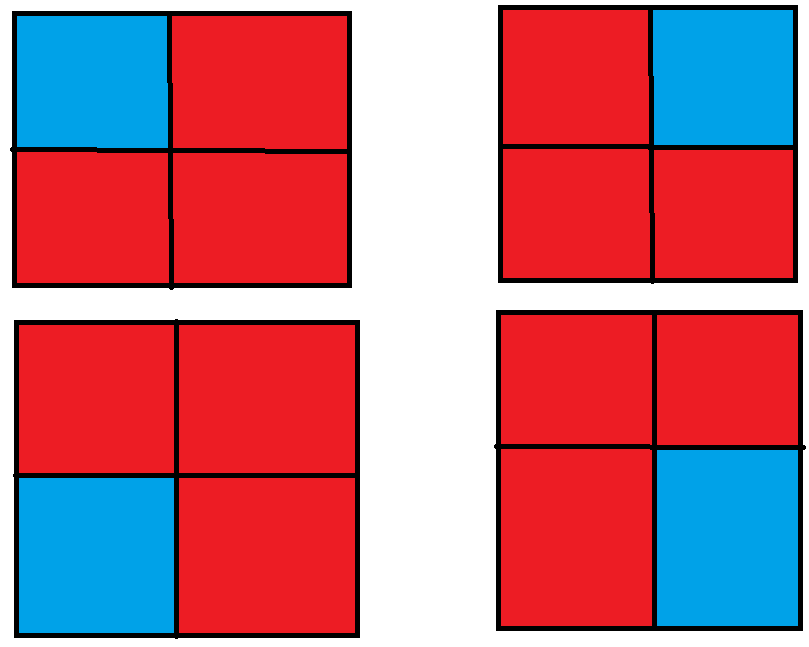
\includegraphics[width=0.45 \linewidth]{triomino_2x2.png} &
	  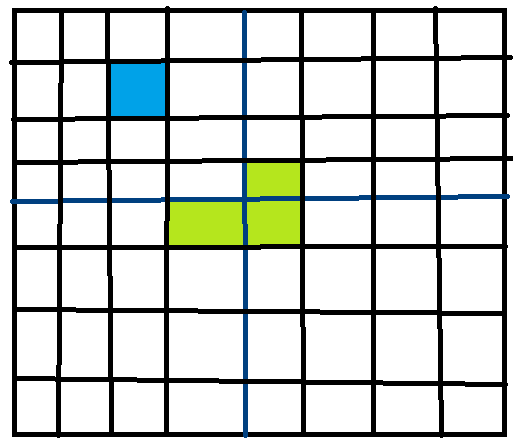
\includegraphics[width=0.45\linewidth] {triomino_2nx2n.png} \\
    (a) & (b) \\
       \end{array} \]
 \end{center}
\caption{(a) Tiling a $2\times2$ square with a tile missing, colored in blue, in four different configurations. The L-shaped square is colored in red. (b) A $8\times 8$ chess board with one square(shown in blue) missing. The L-shape(shown in green) is placed at the center of the board such that it touches each of the three remaining quadrants. }
\label{fig1}
\end{figure}

\vspace{-10pt}

\begin{proof} We prove  the above lemma using the principle of induction.

  {\bf [Basis step]} Assume $n=1$. In Figure \ref{fig1}(a),  we show four different positions of the missing tile(in blue). Each of these configurations can be tiled as shown in the figure. Thus, the above lemma holds true for $n=1$.

  {\bf [Inductive step]} Assume it also holds true for a $2^n \times 2^n$ board with an arbitrary tile missing. Using the principle of induction, if we can prove that this also holds true for a board of size $2^{n+1} \times 2^{n+1}$ our proof will be complete. 

\noindent First, we divide a $2^{n+1} \times 2^{n+1}$ board into 4 halves, each one of dimension $2^n \times 2^n$. The missing tile can lie in any of the 4 quadrants formed. Now, we place a L-shape in the middle of the board, such that each of its 3 squares lie in quadrants which do not have the missing tile. One such representation is shown in Fig. \ref{fig1}(b). Notice that the L-shape is touching each of the remaining 3 quadrants of size $2^n \times 2^n$. Using our previous assumption, we can tile each of these 3 quadrants, assuming the tile within the L-shape is missing. For the quadrant containing the actual missing square, we use the same assumption of tiling $2^n \times 2^n$. Thus, we prove that the entire board of size $2^{n+1} \times 2^{n+1}$ can be tiled. This completes our proof of the given lemma by induction.
\end{proof}

\noindent (b)  
\noindent Let, us define a {\em configuration} structure for each tile on the board A. The {\em configuration} structure has 3 members: \{ points $\bar{a},\bar{b},\bar{c}$, $o_x$, $o_y$ \}. The points comprise the 3 squares of the L-shape, while $o_x$ and $o_y$ are the offsets for position of the tile with reference to the coordinates of the board. 

\noindent {\bf Claim 1:} The total number of existing squares in the board, that is $4^n-1$ is exactly divisible by 3. Thus, the board can be tiled optimally without leaving out any square untiled. 

\begin{proof}
   We use the principle of induction to prove our claim.

\noindent {\bf [Basis step]} When n = 1, $4^n-1 = 4 - 1 = 3$ . Thus, our claim holds true for $n=1$.

\noindent {\bf [Inductive step]} Assume the claim is true for some integer $n > 0$. We now prove that the claim also holds for $n+1$. 

\noindent For $n+1$, $4^{n+1} - 1 = 4.4^n-1 = 4.4^n - 4 + 3 = 4(4^n-1) + 3$. The rightmost part is divisible by 3, according to our assumption. Thus our claim holds true for all integers $n > 0$ .
\end{proof}

\noindent Now, we can apply a recursive algorithm in the same way as in (a), where each time we divide the chess-board $2^n \times 2^n$ into 4 quadrants. Initially, we place a L-square touching the quadrant containing the missing square, as shown in Fig. \ref{fig1}(b). The three tiles of this L-shape are considered to be {\em pseudo-missing} in their three respective quadrants. Next, we recursively tile the 4 quadrants, each of which now has a missing or {\em pseudo-missing} square. The algorithm terminates on a $2 \times 2$ region of the board, which can be tiled as shown in Fig. \ref{fig1}(a).

\noindent Note, this algorithm has two passes. In the first pass, it recursively goes down the dimensions of the board till it hits a $2\times 2$ patch. In the next pass, it fills the patch and recursively fills all such other patches. As the algorithm terminates, we get as an output a tiled $2^n \times 2^n$ chess-board.

\noindent  We run the algorithm with initial arguments ($A$, [x,y]) where $[x,y]$ is the coordinate of the missing tile. Let, $T(n)$ be the complexity of tiling a $2^n \times 2^n$ board. The time complexity $T(n)$ can be formulated as follows:

\begin{equation}
   T(n) = 4T(n-1) + \mathcal{O}(c) \notag
\end{equation}

\noindent Using the Master Theorem, we obtain $T(n) = \mathcal{O}(4^n)$. Also, since the number of tiles excluding the missing one is $4^n-1$, the number of tiles as the output of our algorithm is $\frac{4^n-1}{3}$. 

\noindent {\bf Configuration of tiles}
\noindent Each tile of the board gets labeled with an unique tile number. To get the configuration of the tiles, we look at each connected block having same value and assigning it a particular configuration (There can be total 4 different configurations of L-shaped tile as shown in Fig. \ref{fig1}(a)).

\vspace{10pt}

\noindent 2. Let, $A\left[ 1\dots n\right]$ be an array containing $n$ integers.  To count the number of inversions in $A$, we have to calculate all pair of indices $\left( i,j\right)$ such that $i < j$ and $A[i] > A[j]$. We proceed to count the number of inversions in a divide and conquer method as follows.

\begin{enumerate}
   \item If $A$ has only 1 element, return 0;
   \item Divide  $A$ into  two parts at the middle element.
   \item Call {\emph MergeSort (Left half)} which returns the number of inversions in left half and the sorted left half. Let the number of such inversions be $i_1$.
   \item Call {\emph MergeSort (Right half)} which returns the number of inversions in right half and the sorted right half. Let the number of such inversions be $i_2$.
   \item {\emph Merge} the two halves, which returns the additional number of inversions. In the {\em Merge} process, let $i$ is used for indexing the left sub-array and $j$ for right sub-array. At any step in {\em Merge}, if $A_i > A_j$, then there are $\| middle - i\| $ inversions, because the two sub-arrays are sorted and so all the remaining elements in left sub-array $\left [ i+1, i+2 \dots middle \right ]$ will form inversions with j. Let the number of such inversions be $i_3$.  
   \item return the result as $i_1 + i_2 + i_3$. 
\end{enumerate}

\noindent  In the above algorithm, steps 2 and 3 essentially reduces the search-space equal to half the size of the original array. Finally, in the merging step, we iterate over $n$ elements of the array. Thus, if $T\left(n\right)$ is the time complexity of this algorithm, time complexity of the entire algorithm can be written as:

\begin{equation}
  T\left( n\right) = 2T\left( \frac{n}{2} \right) + \mathcal{O} \left( n\right) \notag
\end{equation} 

\noindent The above equation can be solved in $\mathcal{O} \left( n\log n\right)$ time. Thus, time complexity of our algorithm is $\mathcal{O} \left ( n \log n\right )$.

\vspace{10pt}

\noindent 3. (a) \\
{\bf Standard pancake sorting algorithm:}

\begin{center}
\begin{enumerate}
  \item $current\_size = \left|array\right|$
  \item if $current\_size \le 1$, exit
  \item find index of maximum element in array from $[0, \dots current\_size]$. Let, this index be $m$.
   \item if $m == current\_size$, decrease $current\_size$ by $1$ and goto Step 2.
   \item flip(arr, $m$)
   \item flip(arr,$current\_size-1$)
    \item decrease $current\_size$ by $1$
    \item goto Step 2.
\end{enumerate}
\end{center}

\noindent In the worst case, number of flips is $2n-3$, since the smallest pancake does not require any flip. \\

 (b)

\noindent {\bf Burnt pancake sorting algorithm:}

\begin{center}
\begin{enumerate}
  \item $current\_size = \left|array\right|$
  \item if $current\_size == 1$, flip top pancake, if necessary, such that burnt side is down. exit
  \item find index of maximum element in array from $[0, \dots current\_size]$. Let, this index be $m$.
   \item if $m == current\_size$, decrease $current\_size$ by $1$ and goto Step 2.
   \item flip(arr, $m$)
   \item flip top pancake, if necessary, such that burnt side is up. [If we push the top pancake with burnt side up to the bottom of the stack, then its normal side will be up. Otherwise everytime the burnt side of the maximum pancake will be at the top.]
   \item flip(arr,$current\_size-1$)
    \item decrease $current\_size$ by $1$
    \item goto Step 2.
\end{enumerate}
\end{center}

\noindent In the worst case, the number of flips performed is $3n-2$, since the smallest pancake requires just one flip.

\vspace{10pt}

\noindent 4. (a) The total number of cells in a kd-tree containing $n$ points is $n+1$. 

\begin{proof}
  Drawing a line through each point is essentially adding an extra cell. For example, initially we have just one cell, the entire domain. In the first step of the algorithm, the median point is selected and a vertical line is drawn which splits the entire domain into two cells. In this way, at each step of the algorithm, we are adding a new cell to the tree. Hence, proved.
\end{proof}

\noindent (b) The number of cells a horizontal line can cross is $\mathcal{O}(\sqrt{n})$. The reason is that for the horizontal line drawn, the result is the number of points lying immediately above the height(h) of the line. So, we can look at odd depths of the kd-tree and search for values in the nodes that are greater than h. Thus, at each node we compare h to the node value and move to its grandchildren accordingly. This essentially decreases the search-space by $\frac{1}{4}$. Thus, if $T(n)$ be the number of cells visited from a node, $T(n) = 2T(\frac{n}{4}) + O(c)$. This gives $T(n) = \mathcal{O}(
\sqrt{n})$.


\begin{figure}
  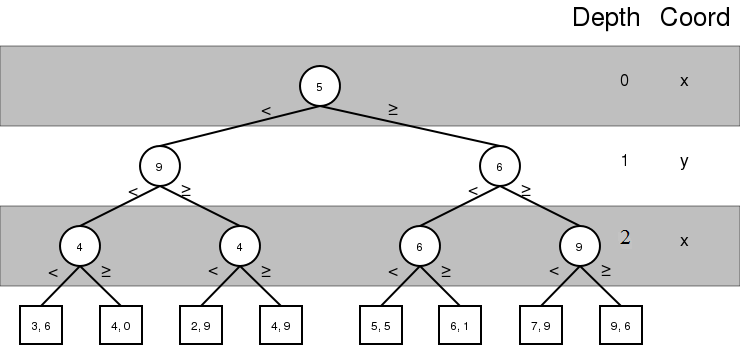
\includegraphics[width=\linewidth]{kdt.png}
   \caption{A sample kd-tree construction given points $\{ (2,9), (3,6), (4,9), (4,0), (5,5), (6,1), (7,9), (9,6) \}$. The kd-tree is constructed by inserting the points at the leaves of the tree. Ref : [http://ldots.org/kdtree]}
\end{figure}


\noindent (c) The question can be restated as finding the number of points in the domain having y-coordinate greater than or equal to the height(h) of the horizontal line. Now, maximum depth of the kd-tree is $\mathcal{O}(\log_{2} n)$. To find points with y-coordinates greater than h, we search over the entire height of the tree. First, let us make two claims.

\noindent {\bf Claim 1} If the value at a node is greater than or equal to h, we can straightaway add the number of leaves in the right subtree of the node to the answer. Next, we need to look only in the left subtree of that node.

\noindent {\bf Proof:}  Since the value at each node is the median of a subset, our search space reduces to points which have y-coordinates less than that at the node. This follows the logic of a binary search in a sorted array. However, all the leaves in the right subtree also add to the result, since all of them have y-coordinates $\ge$ h.

\noindent {\bf Claim 2} If the value at a node is less than h, we can straightaway ignore the left subtree of the node. We only need to look only in the right subtree of that node.

\noindent {\bf Proof:} This follows from the earlier proof.  Here too the search space is reduced to half. All the points in the left subtree of the node will not contribute to the resulting set. 

\noindent With the above claims in mind, we can see that any horizontal (or vertical) line can intersect at most two of the four subtrees associated with the grandchildren of a node. The other two, as shown in the claims will be entirely contained within the halfspace or lie entirely outside the halfspace) At each node of the kd-tree we split the domain in half. Thus, the number of points in each grandchild is $\approx \frac{n}{4}$. Hence, if $T(n)$ be the query time for our algorithm, then $T(n)$ can be formulated recursively as follows:

\begin{equation*}
    T(n) = 
       \begin{cases}
		1, & \mbox{if $n = 1$}, \\
	    2T(\frac{n}{4}) + 1. & \mbox{otherwise}
       \end{cases}
\end{equation*}

\noindent Using Master Theorem, we find the solution  $T(n) = \mathcal{O}(\sqrt{n})$. Therefore, the total time complexity, including the enumeration time, is $\mathcal{O}(\sqrt{n} + k)$, where $k$ is the number of points enumerated in the result.

%\vspace{10pt}

\noindent (d) The solution to this problem involves multiple calls to our query function with different arguments. We first divide the problem into the following parts. Let, rectangle {\emph R} be denoted by x-range : $[x_{min}, x_{max}]$ and y-range : $[y_{min}, y_{max}]$.  We query the kd-tree to return points whose x-coordinates $\ge x_{min}$. Let, this list be $L_{1}$. Second, we query for points with x-coordinates $\le  x_{max}$. Let, this list be $L_{2}$. Similarly, we query for points with y-coordinates $\ge y_{min}$ and $\le y_{max}$. Let, these lists be $L_3$ and $L_4$ respectively. Finally, we find the points at the intersection of these, that is $L = L_1 \cap L_2 \cap L_3 \cap L_4$. The worst case complexity for generating each of these lists is $\mathcal{O}(\sqrt{n} + k)$. Computing the intersection is again $\mathcal{O}(k)$. Therefore, the total time complexity is $\mathcal{O}(\sqrt{n} + k)$.
\vspace{10pt}

\noindent 5. (a) The algorithm to compute the number of elements in $X + Y$ is described as follows: 

\begin{enumerate}
  \item Generate the number of pair of elements from Minkowski sum of sets X and Y. There can be at most $n^2$ of such elements. This operation takes $\mathcal{O}(n^2)$ time.
  \item Sort the resulting array. This takes $\mathcal{O}(n^2 \log n^2) \equiv \mathcal{O}(n^2 \log n)$ time. 
   \item Compress the array such that duplicate entries are removed. This operation takes $\mathcal{O}(n^2)$ .
   \item return length of the compressed array.
\end{enumerate}

\noindent The time complexity of this above method is $\mathcal{O}(n^2 \log n)$. \\

\noindent (b) The naive algorithm, as shown above, can be improved using FFT on the two sets. The resulting algorithm can be described as follows.

\noindent Compute the maximum value in the set $X \cup Y$. Let, this value be $M$. Now, we generate characteristic functions $P[0 \dots M]$ and $Q[0 \dots M]$  for sets X and Y. P and Q are defined according to Eq. \ref{eqn1}.

\begin{equation}
   P(x) = 
     \begin{cases}
            1, & \mbox{if $x \in X$}, \\
             0, & \mbox{otherwise}
      \end{cases}
\hspace{30pt}
     Q(x) =
        \begin{cases}
            1, & \mbox{if $x \in Y$}, \\
             0, & \mbox{otherwise}
         \end{cases} 
\label{eqn1}
\end{equation} 

\noindent It is to be noted that P and Q are of sizes $M+1$. Next, we use FFT method to obtain the convolution of arrays P and Q in $\mathcal{O}(M \log M)$. Let, the resulting convolution array be R. Finally, we scan R to generate a list(L) of indices of each non-zero element.  L is the desired output of our algorithm. The reason behind this inference is that only elements in the Minkowski sum of X and Y will generate non-zero entries in R. Mathematically,

\begin{eqnarray}
  & R(i) \neq 0 \; if  \; \exists k \; s.t. \; P(k) \neq 0 \; and \; Q(i-k) \neq 0  \\ \notag
\implies & R(i) \neq 0 \; if \; \exists k \; s.t. \; k \in X \; and \; i-k \in Y \notag
\end{eqnarray} 

\noindent Since $\left | R \right| = \mathcal{O}(M)$, we can generate list L in $\mathcal{O}(M)$ time complexity. Thus, overall complexity of the algorithm is $\mathcal{O}(M \log M)$.

\end{document}


